\section{Plant as sensor}

\subsection{Technical choices}

%TODO: Rework the technical choices part.
Before diving into the implementation, several technical choices were made to shape the overall design of the system. The first major decision was selecting the ESP32 microcontroller as the core processing unit due to its versatility, offering built-in WiFi, multiple GPIO pins, and analog-to-digital converters, which allow for handling sensor data and wireless communication efficiently.

Additionally, the system's audio capabilities were a critical consideration, leading to the inclusion of a basic amplification circuit to boost sound output, ensuring compatibility with external speakers. The design also included a micro-SD slot to allow for expandable storage, enabling future enhancements like storing pre-recorded sounds or more detailed data logs. These foundational decisions laid the groundwork for a scalable and reliable system, ensuring smooth integration of the components that follow in the implementation.

\subsection{The electronic interface}

The electronic interface is the interface that allows a compute unit to capture and interpret the plant signal and
communication. The interface is a device made by us for this use case. The printed circuit board (PCB)
device is composed of 3 main parts:
\begin{itemize}
    \item The core of the circuit, the microcontroller, an ESP32 Wroom 32
    \item An electronic filter connected using an electrode to the plant
    \item A sound part of the PCB that is including an audio amplifier, a volume knob and a terminal block to connect a speaker
\end{itemize}

The design of the PCB has been done using the open source software Kicad.
As said previously, the circuit contains 3 parts.

The core of the circuit is the computation part, including the microcontroller, an ESP32. All the other
devices of the circuit are connected to the ESP32. The choice to use a devkit has been done 
to ease the electronic conception and to avoid any communication and soldering issue with the MCU\footnote[1]{Microcontroller Unit}.

\begin{figure}[h!]
    \centering
    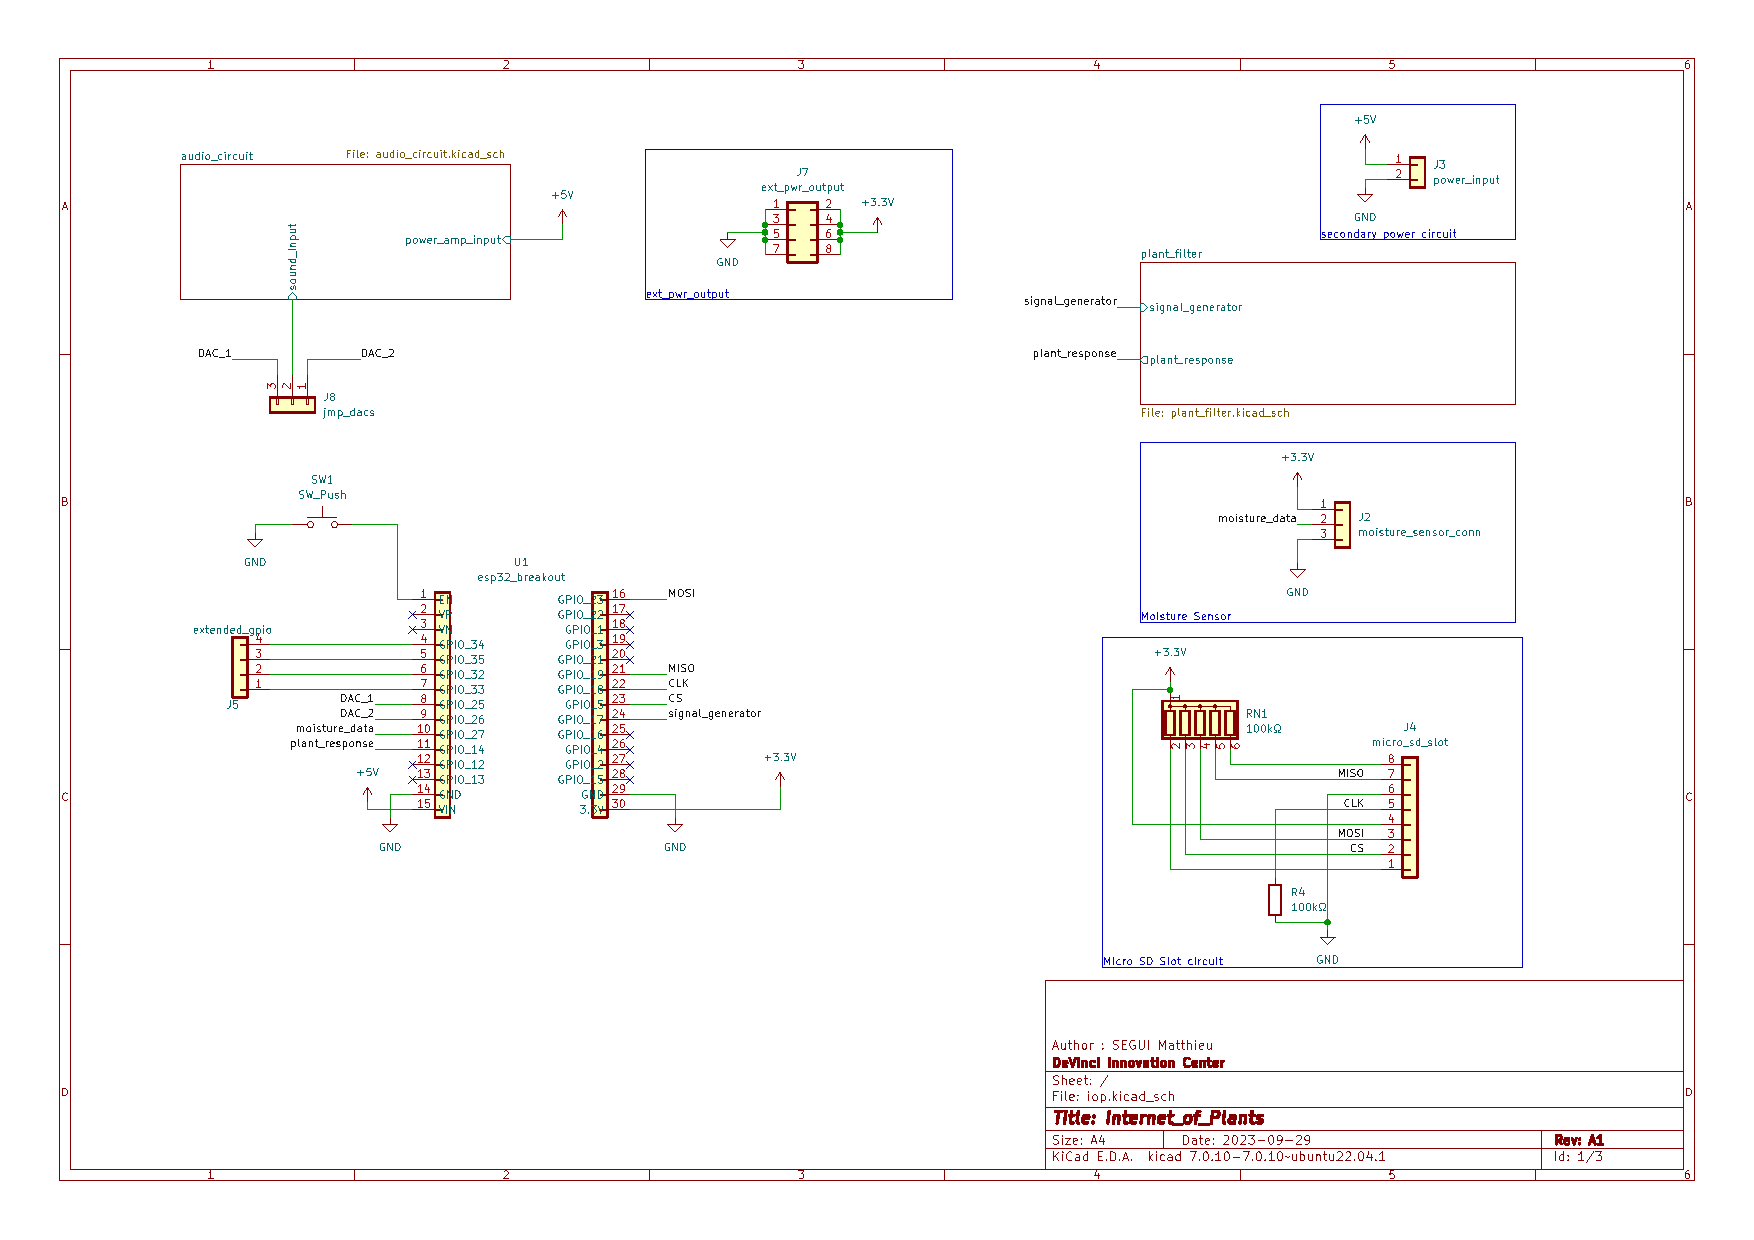
\includegraphics[width=\textwidth]{images/iop.pdf}
    \caption{The main schematic of the device. This main schematic regroups components and sub-sheets (including the audio circuit
    and the filter circuit). The main component is an ESP32 Wroom DevKit. All other components are linked to this
    microcontroller} 
    \vspace{0.1cm}
    \label{fig:iop_schematic_main}
\end{figure}

%TODO: Talk about the humidity sensor

The circuit component that allows us to read data from the plant is the electronic filter.
This filter has been designed by \textit{Jakub Nikonowicz} and \textit{Łukasz Matuszewski} 
from \textit{Politechnika Poznańska}.
Thanks to them, I adapted it for my application on my embedded device. 

\begin{figure}[H]
    \centering
    \includegraphics[width=\textwidth]{images/iop-plant_filter.pdf}
    \caption{The electronic circuit designed to capture the interaction by analyzing the electronic
    frequency response. The circuit includes 3 resistors, 3 inductors and 3 capacitors as main components} 
    \vspace{0.1cm}
    \label{fig:iop_schematic_filter}
\end{figure}

This filter is ending by a crocodile clamp that is directly connected to the plant.

The last part of the circuit is the sound output/rendering. This circuit includes a small amplifier,
the LM386 from Texas Instruments. The rest of the circuit are components needed in order to 
induce amplification on the signal without creating to many noise and saturation.

\begin{figure}[H]
    \centering
    \includegraphics[width=\textwidth]{images/iop-audio_circuit.pdf}
    \caption{The sound output part of the circuit that is used to render the sound. 
    This part includes a small amplifier, the LM386. The circuit also includes the components necessary
    to control and handle the amplification (reduce noise and saturation)} 
    \vspace{0.1cm}
    \label{fig:iop_schematic_audio}
\end{figure}

The PCB is built to be able to add a micro-SD slot (ref to \ref{fig:iop_schematic_main}). This micro-SD slot
allows to increase the storage of the embedded ROM. This can be used to store pre-built sounds and music to avoid generating a sound on-board.  


Once the schematic was completed, the next step was routing the tracks. There are several methods for PCB routing, including single-sided, double-sided, and multiple-layer designs. We opted for a double-sided PCB on each side because this configuration simplifies component placement, making the layout more efficient and organized. Additionally, it is significantly more cost-effective compared to multi-layer PCBs, striking a good balance between performance and budget. Indeed, in terms of routing, PCBs can be single-sided, double-sided, or multi-layered. Single-sided boards are simple and low-cost but limited in complexity. Double-sided PCBs, with copper on both sides, allow for more efficient routing and are commonly used for moderate complexity. Multi-layered PCBs offer even greater routing density, suitable for advanced electronics such as computer motherboards or phone components.

In terms of track width, we used 0.2mm wide tracks for data signals to maintain signal integrity, while the power tracks were designed with a width of 0.8mm. This wider width ensures that the power tracks can safely handle up to 800 mA, providing sufficient current capacity without overheating or voltage drops.

\begin{figure}[H]
    \centering
    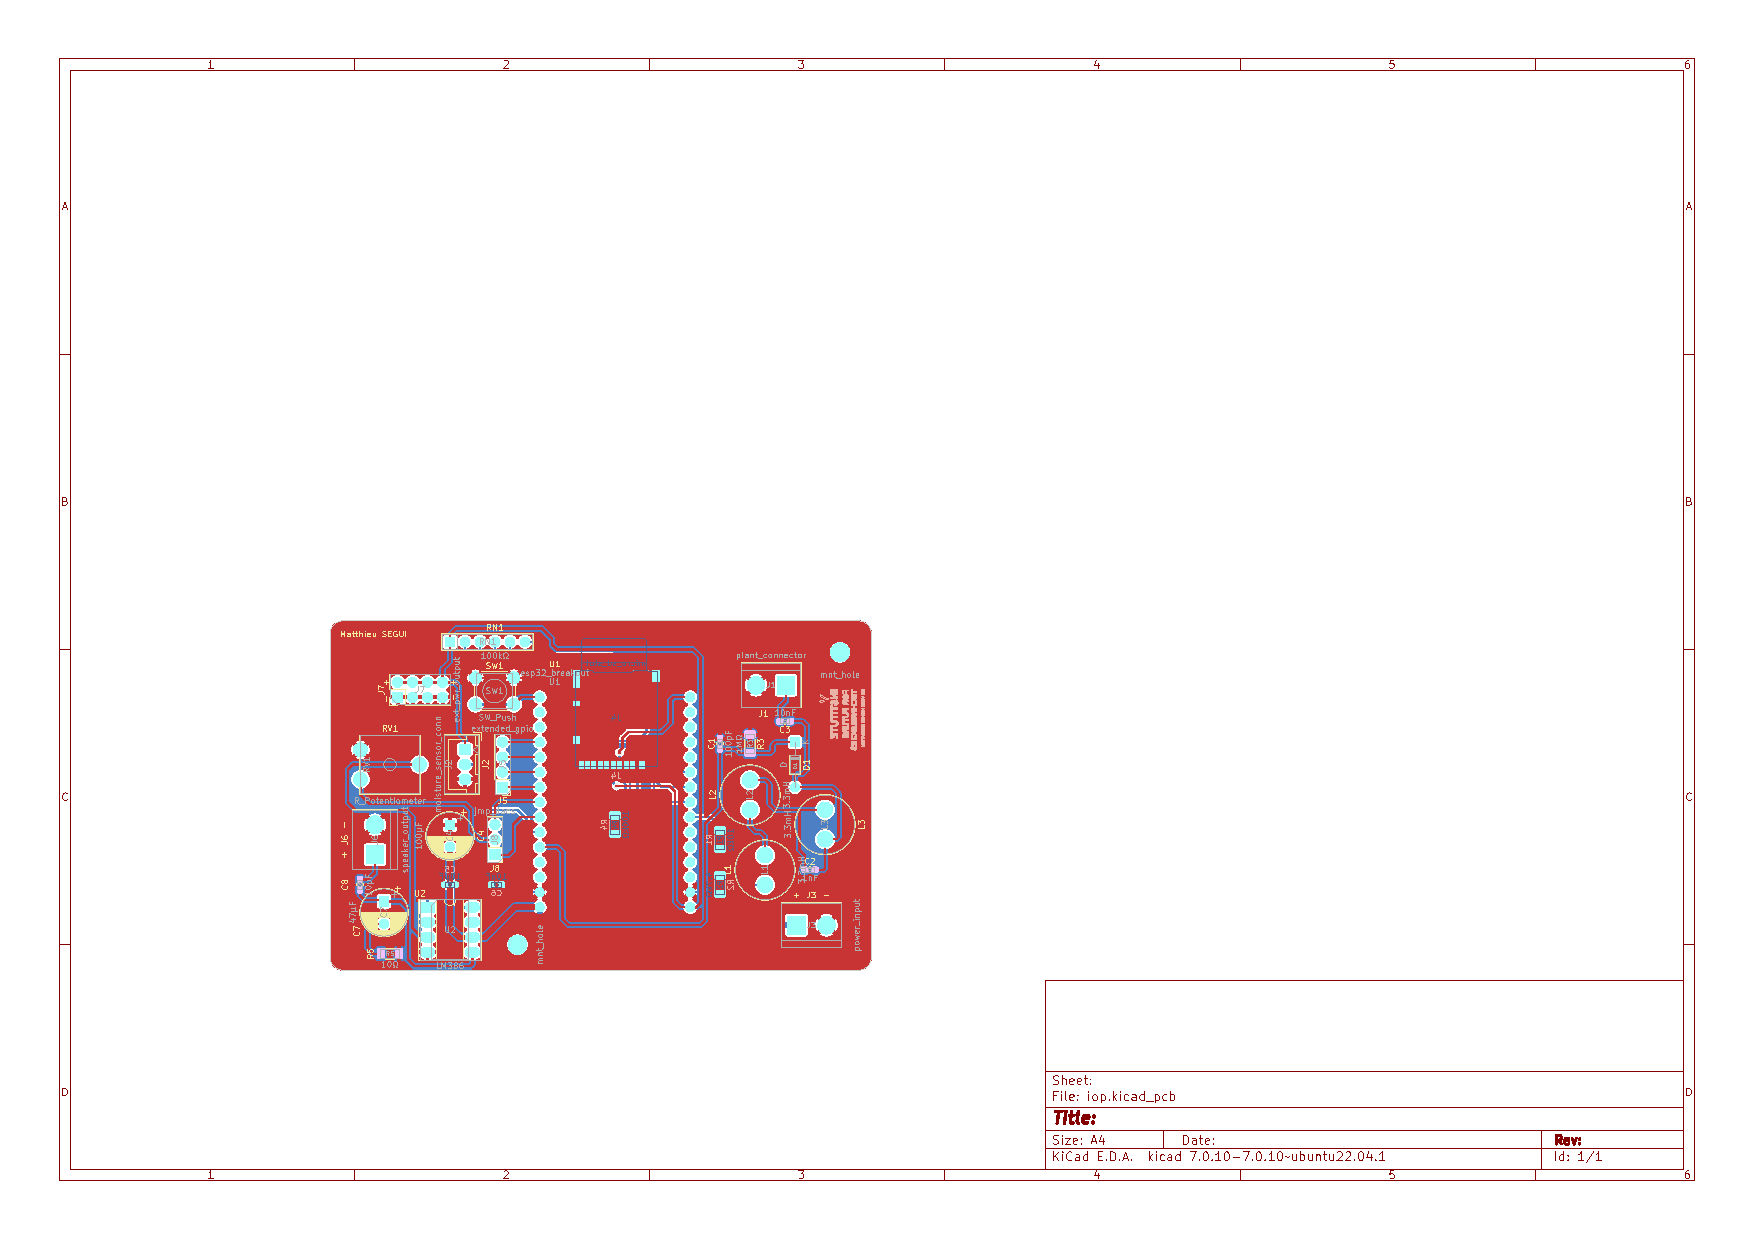
\includegraphics[width=\textwidth]{images/iop-routed_pcb.pdf}
    \caption{Double sided PCB routed. This view allows to see the track used for components inter-connection. The tracks width is 0.2mm for data tracks and 0.8mm for power tracks.} 
    \vspace{0.1cm}
    \label{fig:iop_routed_pcb}
\end{figure}

Kicad also allows us to generated a 3D view of the future PCB. This allows us to imagine what the
PCB will look like when it will be manufactured.
\begin{figure}[H]
    \centering
    \includegraphics[width=0.8\textwidth]{images/front_iop_3D_view_modified.png}
    \caption{Front 3D rendering of the built PCB. The rendering is done using open source software: Kicad} 
    \vspace{0.1cm}
    \label{fig:front_iop_3D_view_modified}
\end{figure}

\subsection{Human interaction}

\subsubsection{Use of the sensor/filter}

The device is able to capture the human interaction with the plant. The touch interaction is inducing changes
in the impedance, capacitance and inductance of the plant. Values are captured using the GPIO (General Port Input/Output)
14 of the ESP32 DevKit. This GPIO is able to read analog data and convert them to digital values using analog to digital
converter (ADC). The values are a floating point number between %TODO: Add the range of the values here.
Values are fluctuating depending on the interaction. 

%TODO: Add a table comparing the values depending on the interaction

The possibilities of 


\subsubsection{Sonification on the device} % FIXME: subsubsection ??

The human interaction goes through the sonification on the device. ESP32 embeds a 8-bit digital to analog converter (DAC).
The embed DAC is enough to play low quality sounds. Combined with the micro-SD card including in it, it is a media player.
Using the \textit{Arduino Audio Tools} library it is possible to read MP3, Wav and other audio format.
Taking the sensor value as an input, you can then apply a pitch shift on the data that will be rendered on the DAC.
The pitch shift is a value included between 0 and 100. We are mapping the max value of the sensor and the min value
to this range using the \textit{map()} Arduino function.

The data is sent to the DAC and rendered. \textit{Arduino Audio Tools} also includes a way to communicate data to the
DAC.

%TODO: Add oscilloscope screenshot of the sound output.

There are two DAC available on the ESP32. DAC 1 and DAC 2 respectively on GPIO25 and GPIO26. The IoP device allows
to choose between the one you want by using a removable jumper.

The output of the DAC is too low to be able to render it on a speaker. The amplification circuit allows a small 
amplification of the output. The amplifier is a basic and simple one. I added a 10k Ohms potentiometer to be able to
tweak the volume. The sound quickly reach amplifier limitations and is becoming saturated. 

The amplified output is sent to a terminal block that acts as the connection interface to the audio speaker.
The audio speaker chosen in our specific example is a 8 Ohms 3 Watts speaker. 

\begin{figure}[h!]
    \centering
    \includegraphics[width=0.6\textwidth]{images/speaker.jpg}
    \caption{8 ohms 3 Watts basic speaker used in our example.} 
    \vspace{0.1cm}
    \label{fig:speaker}
\end{figure}


\newpage
\subsubsection{User study}
\paragraph{Abstract of user study}
This study explores human-plant interaction.
This study has been conducted in order to understand what kind of interaction we have to detect in order to have the best and more natural kind of interaction with plants.
The results will be applied in the Internet of Plants (IoP) project which intends to create a fully connected bio-organ system.
The IoP is looking to reduce the gap between humans and plants by creating a symbiotic relationship between 
nature and technology. We envision a world where our daily objects are responsive.

\paragraph{Introduction}
Plants represent a full ecosystem of evolution, adaptation and communication.

In the context of the Internet of Plant (IoP) project, this study aims to extract the natural interaction between people and plants.
This experiment explores the interactions the IoP device will have to detect to create a symbiotic relation between human and plants. 
The physical touch is the starting point of a sonification process.
Sonification is “the use of non-speech audio to convey information or perceptualize data” \cite{kramer2010sonification}.
Three distinct plant species—\textit{Dypsis lutescens, Pachira glabra, and Dracaena}—are employed as subjects to extract user perceptions and interactions within this framework. 

The methodology engages students from the engineering school and two researchers.
The participants are asked to interact with the plants and imagine the sounds that could be generated by the plants.

The correlation between plant height and trunk interactions reveals environmental factors impacting human-plant dynamics.
Additionally, interactions are categorized based on intensity, spatial displacement, and duration.


\paragraph{Methodology}

\subparagraph{Participants}
The study is conducted on 22 participants. Participants are mainly composed of engineering students. The participant set includes 15 males and 7 females.
The age of participants is between 19 and 22 years old. Exception for three participants that are older than 22 years old. 




\subparagraph{The Procedure} 
We introduced the subject telling participants : 
"We're in the very near future. You are looking at plants that make music when you physically interact with them (it is not actually the case, but imagine it). Explore their capabilities."
Using this prompt, we tried not to bridle them to much but approach them to the physical interaction component.
Subsequently, participants were given time to explore the potential musical capacities of the plants at their own pace.
We conducted the study without providing any guidance during the exploration phase.
In instances where participants encountered difficulty initiating exploration, the prompt was reiterated to encourage the participants to explore.
This methodological approach was designed to capture the intuitive and natural human-plant interaction.
Also, we avoided any kind of communication or talking between 2 participants to reduce the potential bias.


\subparagraph{Materials/Tools}

To proceed and conduct this user study, we chose 3 different plants from 3 different species.


\textit{\textbf{Dracaena}}: It has long leaves and fragile perceived trunk but also flexible. The plant is 95 cm tall.

\begin{figure}[h!]
    \centering
    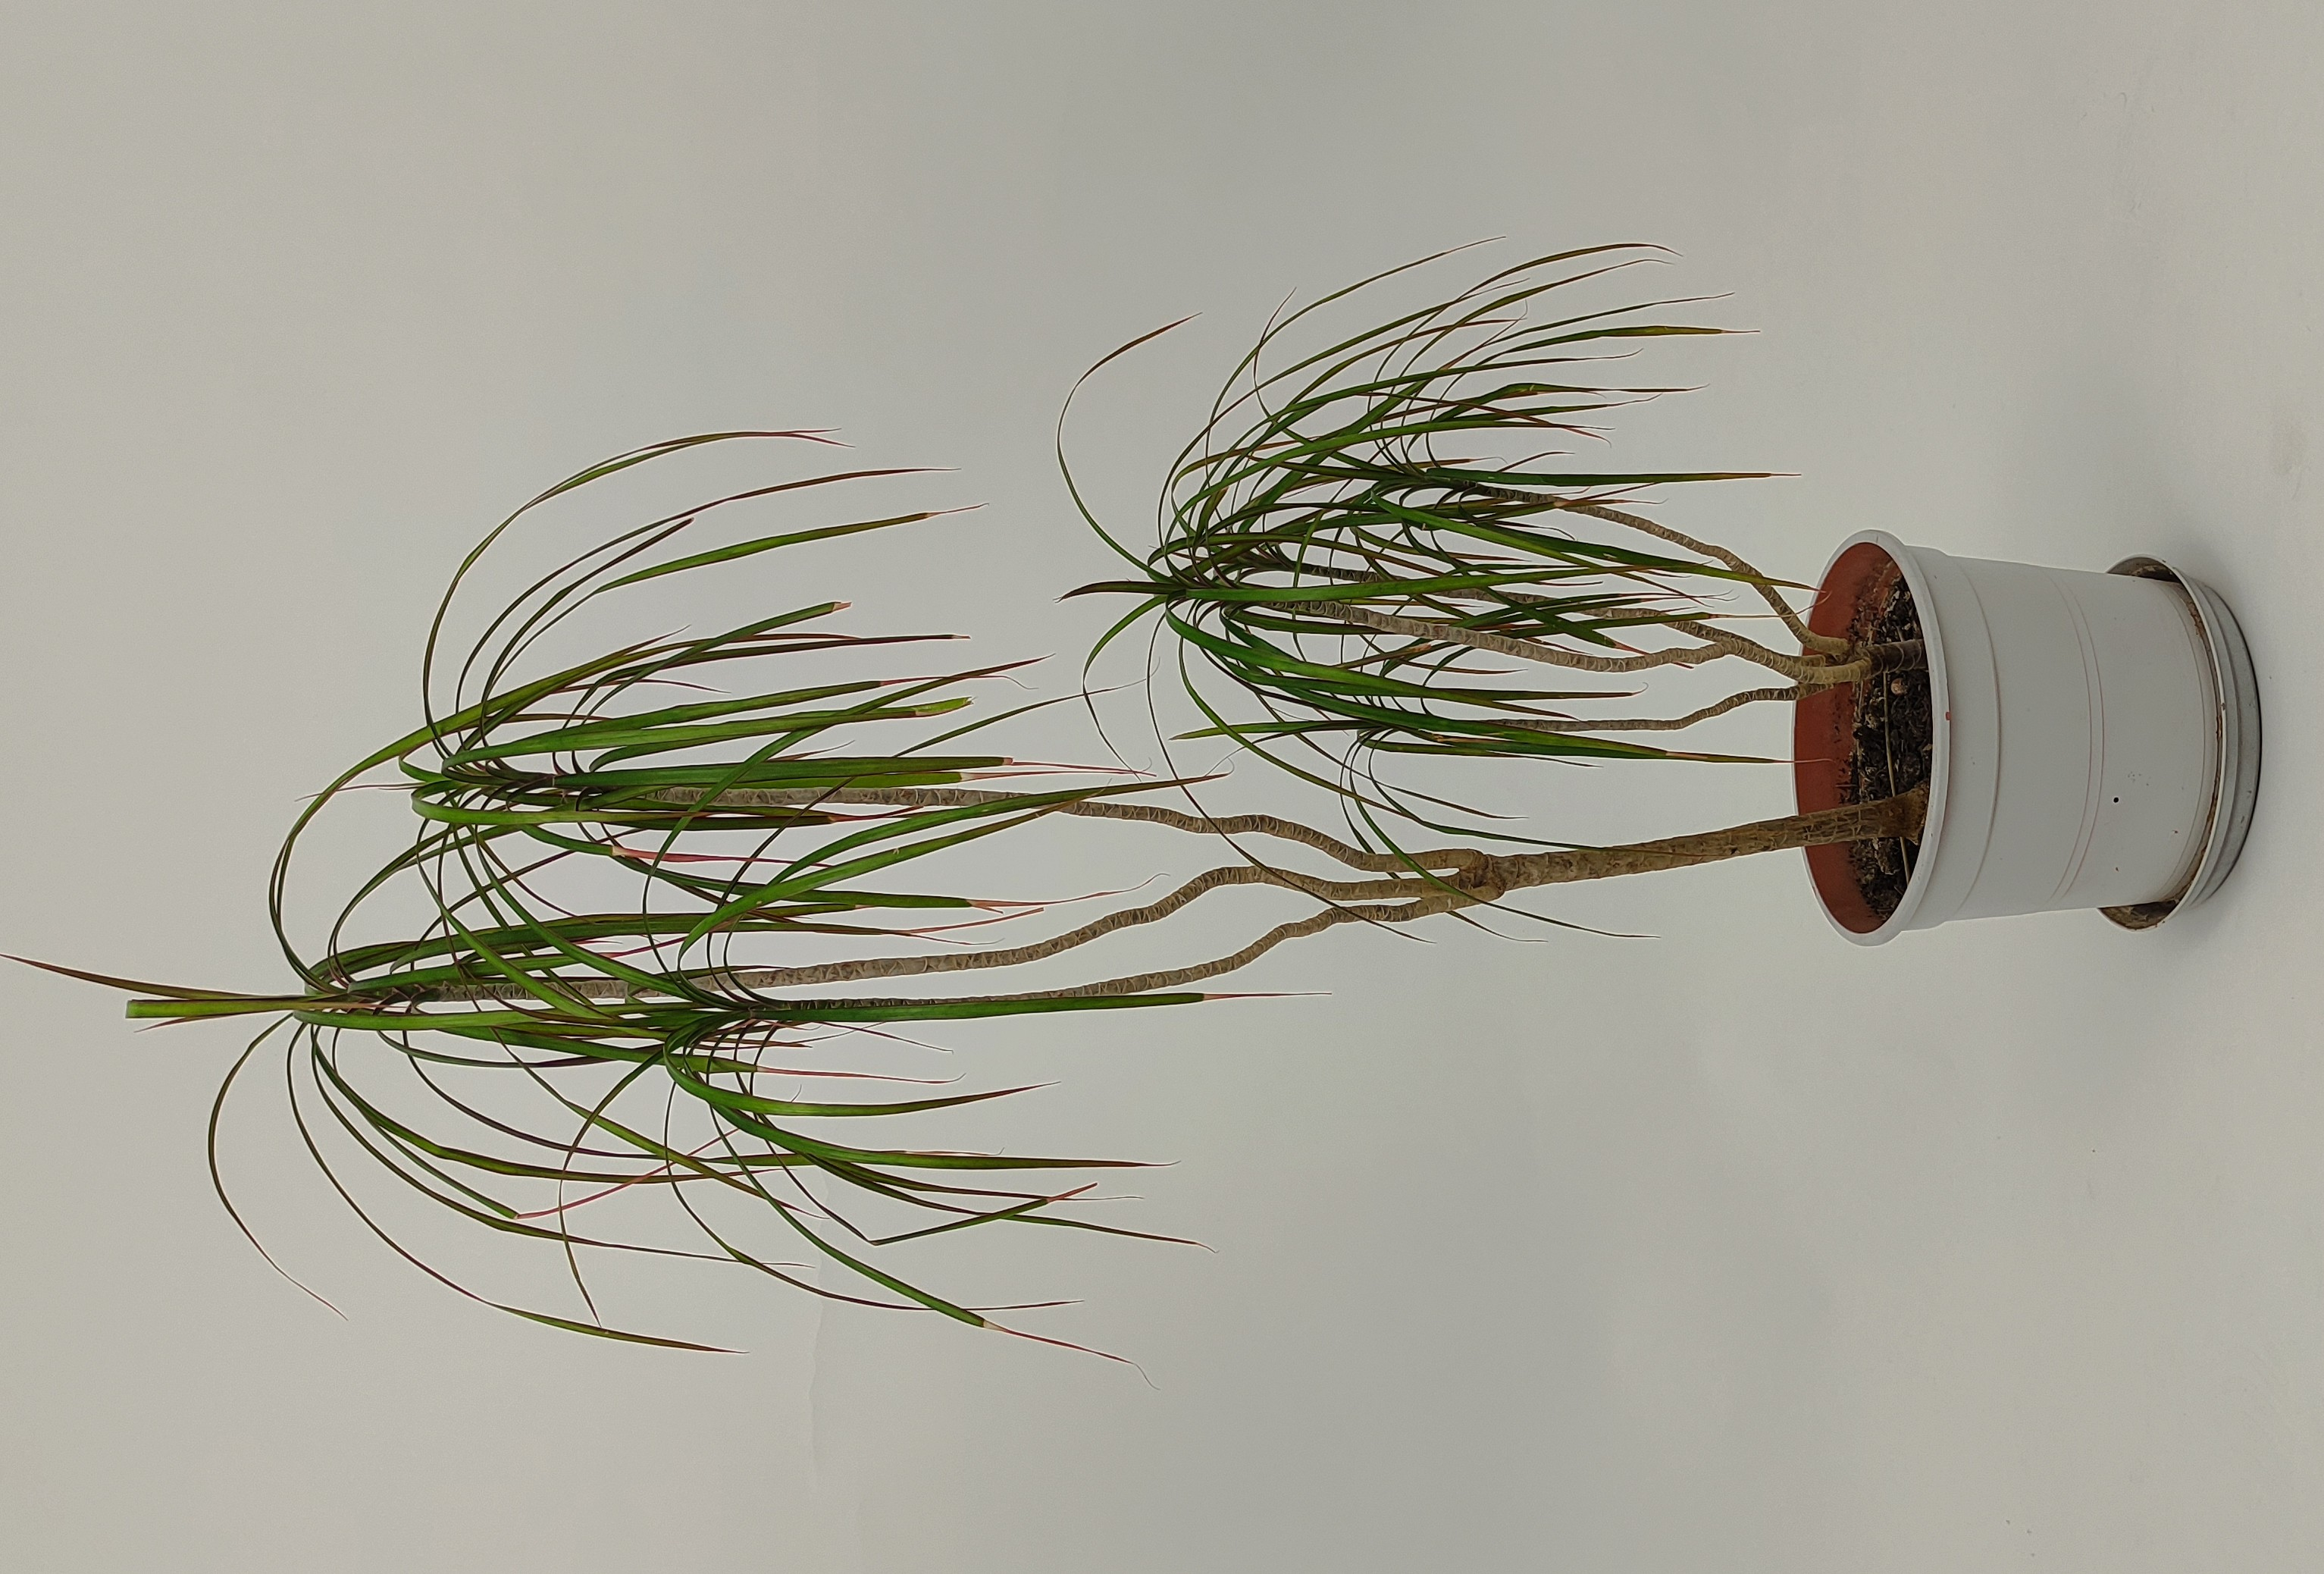
\includegraphics[width=0.8\textwidth, angle=-90]{small_plant.jpg}
    \caption{The N°1 plant is a \textit{Dracaena}.}
    
    \vspace{-0.5cm}
    \label{fig:small_plant}
    \vspace{0.2cm}
\end{figure}




\textit{\textbf{Pachira glabra}}:We chose to use this plant for its large leaves and its wide trunk.
The plant is 110 cm tall.

\begin{figure}[h!]
    \centering
    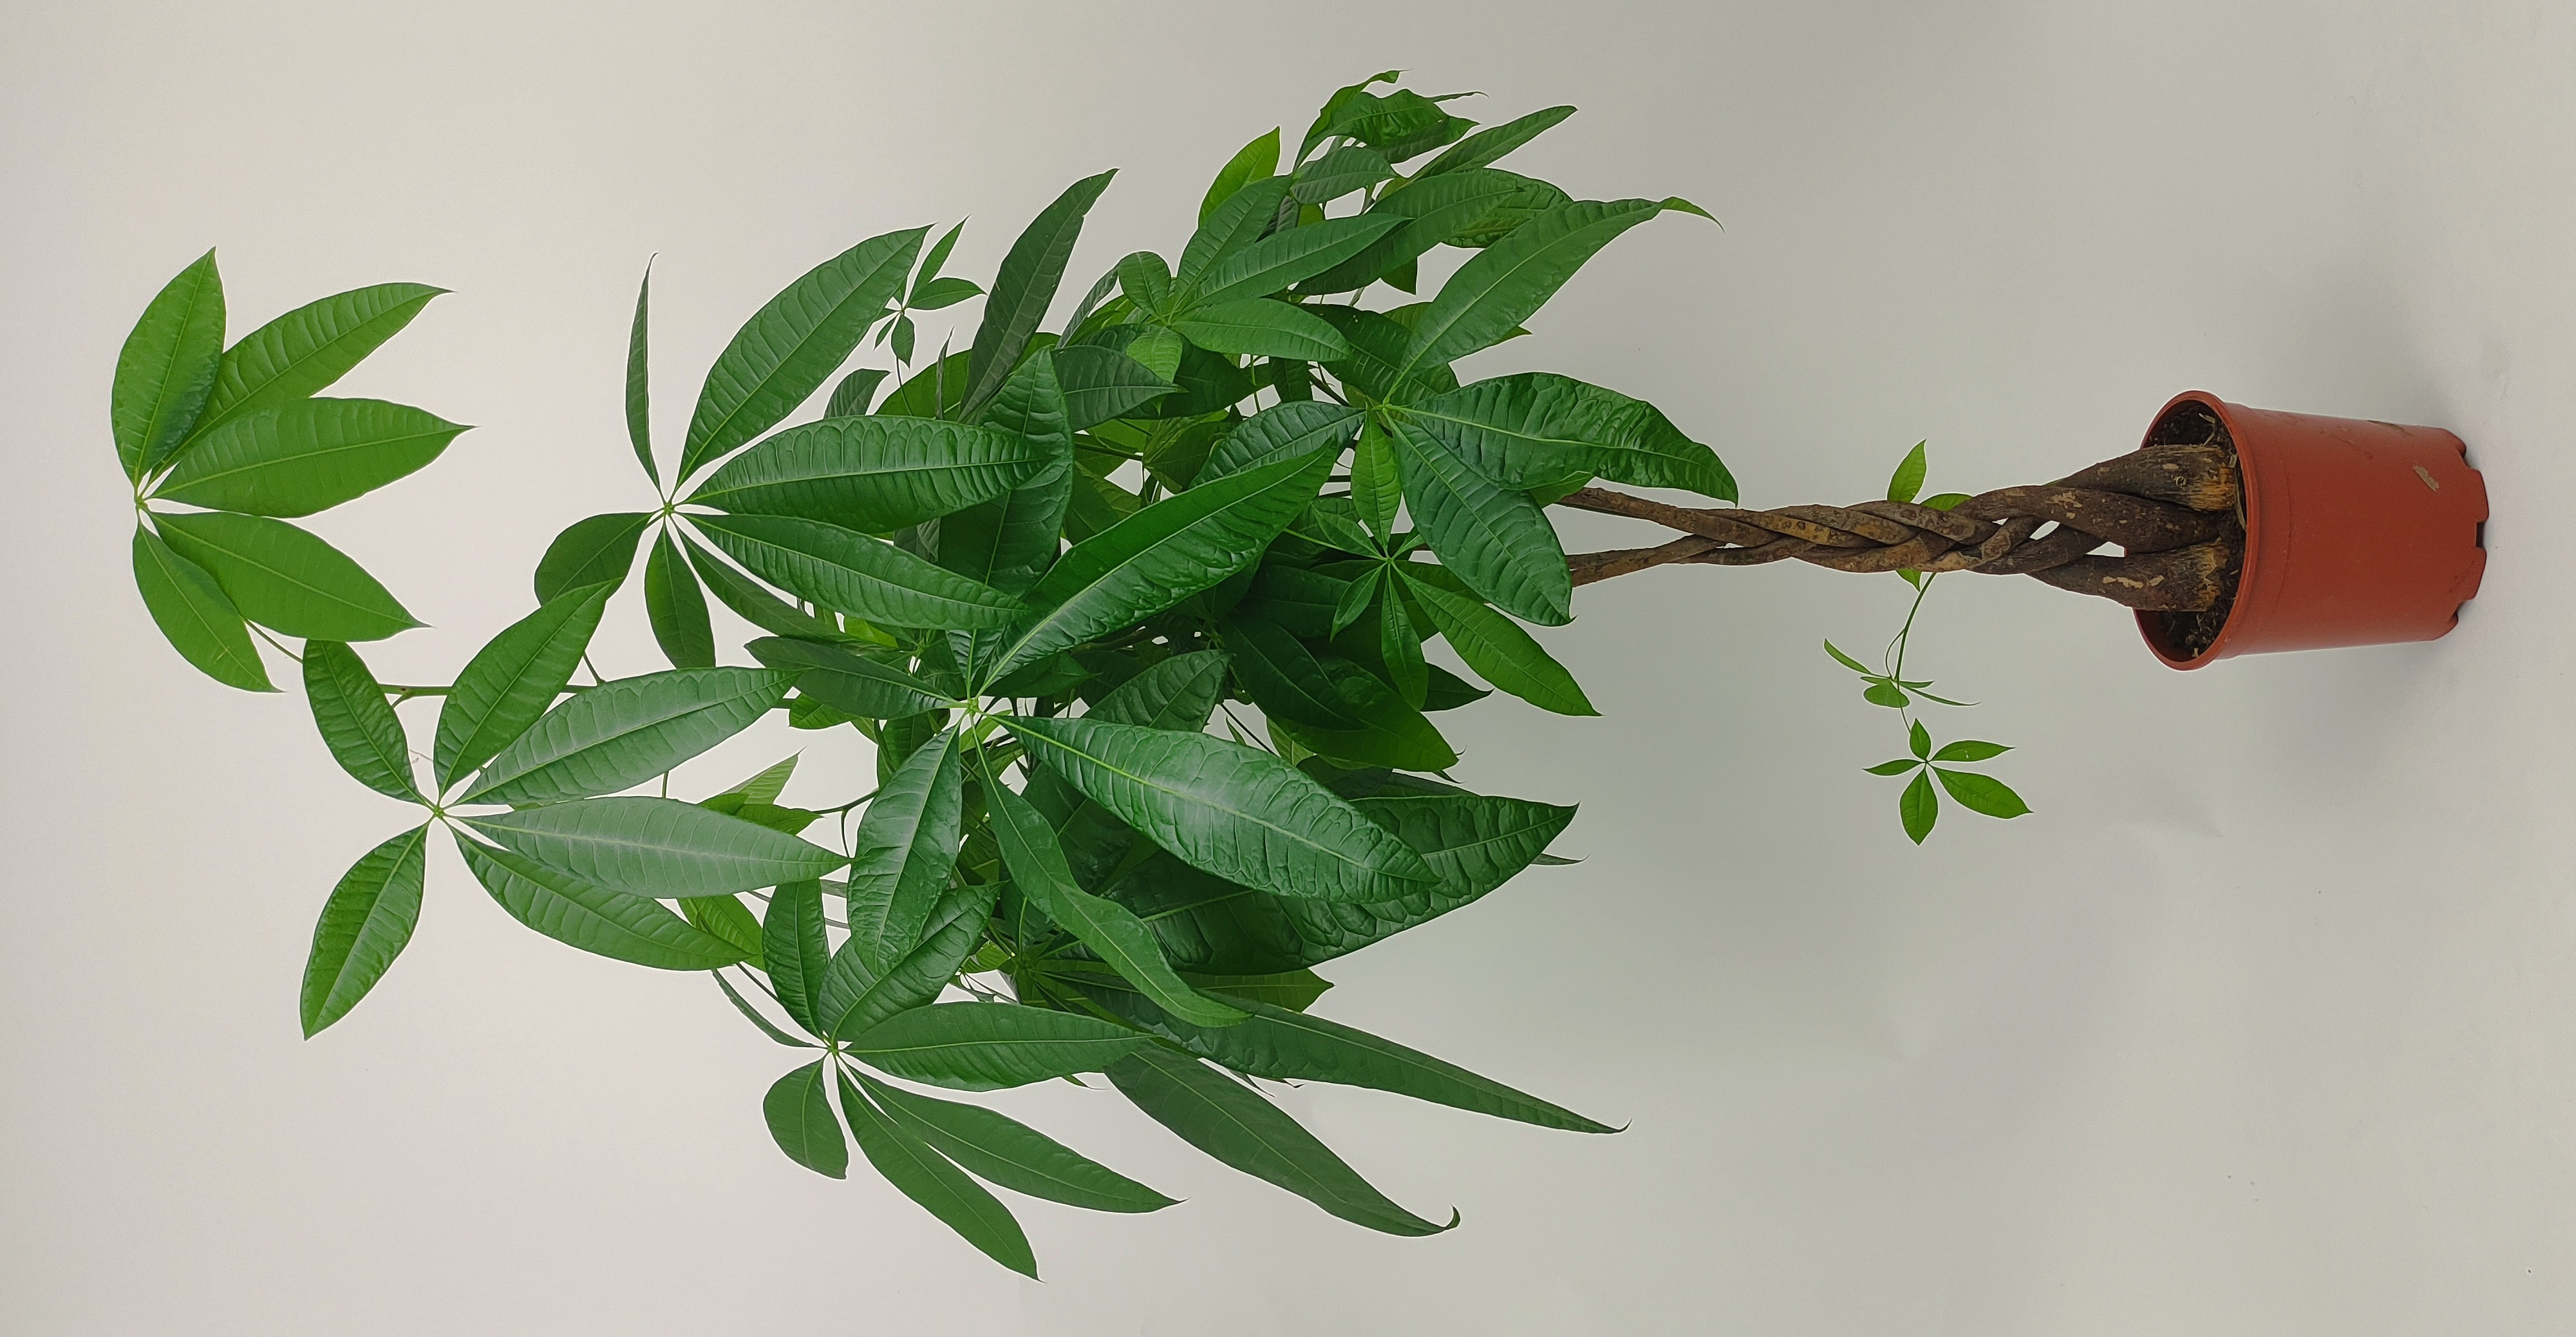
\includegraphics[width=0.8\textwidth, angle=-90]{tall_plant_cropped.jpg}
    \caption{The N°2 plant is a \textit{Pachira glabra}.}
    
    \vspace{-0.5cm}
    \label{fig:tall_plant}
    \vspace{0.2cm}
\end{figure}



\textit{\textbf{Dypsis lutescens}}: The \textit{Dypsis lutescens} is composed of many trunks and stems. On top of that, the leaves are numerous and tight. The plant is \hl{...} tall.

\begin{figure}[h!]
    \centering
    \includegraphics[width=0.8\textwidth, angle=-90]{fougere_plant.jpg}
    \caption{The N°3 plant is a \textit{Dypsis lutescens}.}
    
    \vspace{-0.5cm}
    \label{fig:fougere_plant}
    \vspace{0.2cm}
\end{figure}



\subparagraph*{The experimental space}
The experimental space featured three distinct levels of height, each corresponding to one of the three plants introduced to participants.

\begin{figure}[h]
    \centering
    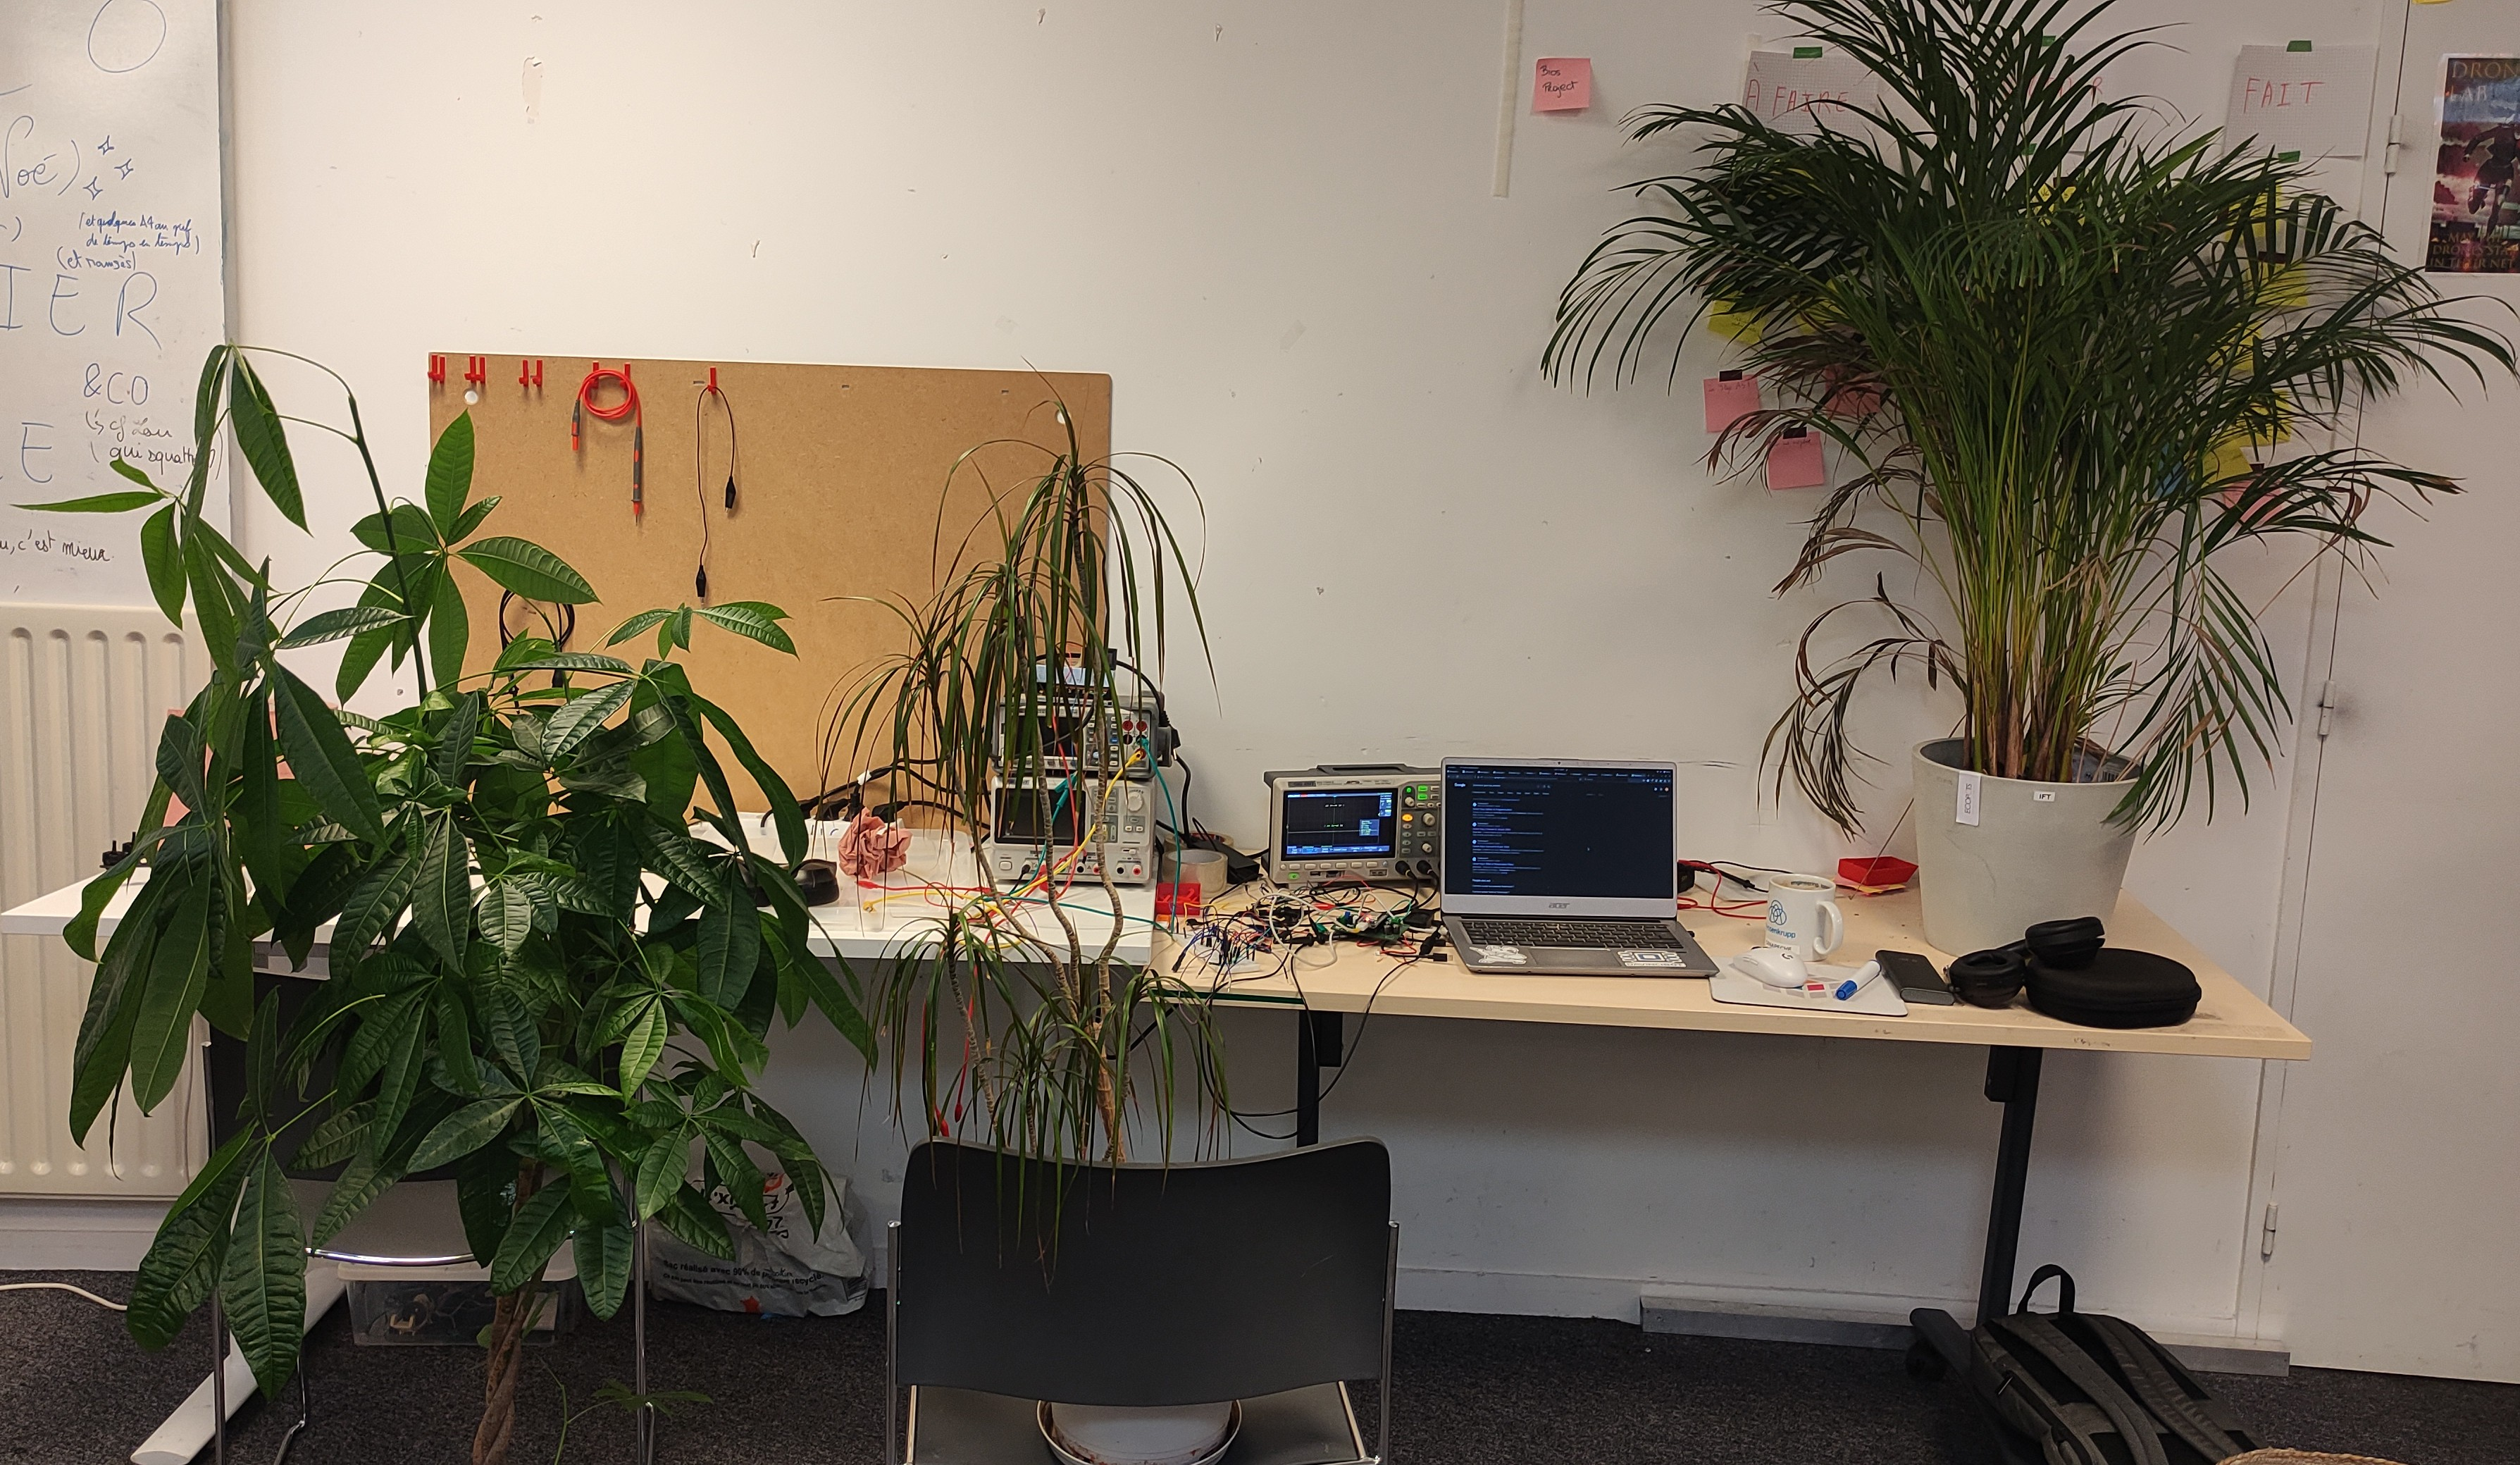
\includegraphics[width=0.8\textwidth]{setup_user_study.jpg}
    \caption{User study space setup. The setup is built from our lab space.}
    
    \vspace{-0.5cm}
    \label{fig:setup_user_study}
    \vspace{0.2cm}
\end{figure}

\paragraph{Data collection}
To capture the participant's interactions with the plants, a collaborative approach was adopted, involving two researchers to provide dual perspectives.
Throughout the exploration phase, both researchers took notes, documenting the diverse ways in which participants engaged with the three distinct plants.
The researchers explicitly specified the plant involved in the interaction in order to extract special features related to a specific plant.

The written notes retrieved descriptions of participants' actions, movements and interactions.
The dual-observer strategy tends to reduce the potential biased.

At the beginning of the experiment, the \textit{Dypsis lutescens} was on the floor, the \textit{Dracaena} was on a chair and the \textit{Pachira Glabra} was on a table.
At the middle of the experiment, we switched the \textit{Dypsis lutescens} and the \textit{Pachira Glabra} to see if the participants would interact differently with the plants.
The set-up of the experiment is shown in Figure \ref{fig:setup_user_study}. 


\paragraph{Results}

The data given by the user study allowed us to define 5 main types of interaction. Those interactions are defined by the way the user interacts with the plant. The 5 main types of interaction are :

\begin{itemize}
    \item Grasp : user uses the whole hand to grab trunk or leaves.
    \item Pinch : user uses 2 to 3 digits to grab trunk or leaves.
    \item Slide : user uses his/her hand or finger to slide on the plant whether is on a leave or on the trunk. The action is continuous.
    \item Pet : user uses his/her hand to cuddle the plant or to pass through the leaves. The user is moving his/her hand in space. She/he is not staying still or staying on a particular object.
    \item Tam Tam : user taps on the plant mainly using the whole hand.
\end{itemize}



Looking at the results, we extracted the table \ref{tab:results}.


\begin{table}[ht]
\begin{tabular}{|l|ll|l|ll|}
\hline
\multirow{2}{*}{Plant/Interaction} & \multicolumn{2}{l|}{Group 1}       & Group 2 & \multicolumn{2}{l|}{Group 3}       \\ \cline{2-6} 
                                   & \multicolumn{1}{l|}{Grasp} & Pinch & Slide   & \multicolumn{1}{l|}{Pet} & Tam Tam \\ \hline
Plant N°1                          & \multicolumn{1}{l|}{4}     & 8     & 4       & \multicolumn{1}{l|}{4}   & 2       \\ \hline
Plant N°2                          & \multicolumn{1}{l|}{9}     & 3     & 3       & \multicolumn{1}{l|}{3}   & 10      \\ \hline
Plant N°3                          & \multicolumn{1}{l|}{10}    & 1     & 5       & \multicolumn{1}{l|}{7}   & 3       \\ \hline
Total                              & \multicolumn{1}{l|}{23}    & 12    & 12      & \multicolumn{1}{l|}{14}  & 15      \\ \hline
\end{tabular}
% \caption*{Plant N°1 : Petite | Plant N°2 : Grande | Plant N°3 : Fougère}
\caption{Raw results extracted from the user study}
\label{tab:results}
\end{table}


With the extraction of the result we were able to design a bar chart.
The graph is grouping the interactions by plant. The height of the bar is the number of participants that performed the interaction.
The graph is shown in figure \ref{fig:setup_user_study}.


\begin{figure}[ht]
    \centering
    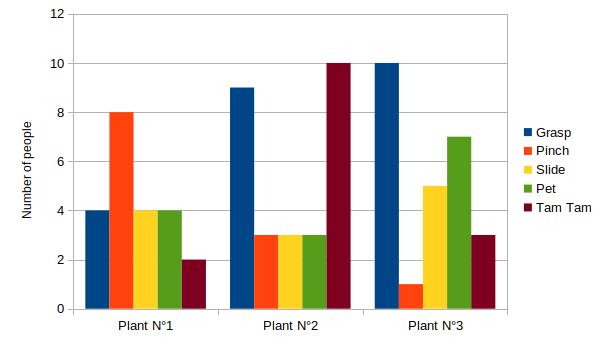
\includegraphics[width=\textwidth]{plant_interaction_chart_2.png}
    \caption{Bar chart that is extracting the main types of interaction regarding each plants.}
    
    \vspace{-0.5cm}
    \label{fig:chart_interaction}
    \vspace{0.2cm}
\end{figure}

In the end, of the 22 participants, 15 were already familiar with the project and 7 were not.

\paragraph{Discussion}
Looking at the results, the interaction were various depending on the plant. 
Thus, we can extract main interactions that are linked to the plant type. 
Looking at table \ref{tab:results}, people are more inclined to use their hands as tam tam or grasp the \textit{Pachira glabra}. 
However, for the \textit{Dracaena} users prefer to pinch the trunk or leave. 
Participants decided to grasp whether a pack of trunk or leaves when it came to \textit{Dypsis lutescens}.
This is induced by many factors including the leaves shape, the width of the trunk.


It was observed that when the plants were positioned at higher elevations on the table, individuals tended to engage more with the trunk of the plants.

Looking at table \ref{tab:results}, we decided to group interaction. This was done by grouping type of interaction depending on 3 main factors :

\begin{itemize}
    \item The intensity factor : what is the intensity of the interaction (ex : pinch is lighter than grasp)
    \item The spatial factor : what is the interaction displacement.
    \item The duration factor : what is the interaction duration (ex : tam tam is instantaneous).
\end{itemize}

The "Group 1" includes the pinch and grasp interaction. Indeed, looking at the 3 factors we defined, 
the pinch and grasp are high in intensity and long in duration but people stay still in space.
This group of interaction can be defined as \textbf{binary interaction}. The user is either grasping or not.

The "Group 2" includes the slide. The slide interaction is long in time, it moves in space but low in intensity.
This group of interaction can be defined as \textbf{continuous interaction}.


Whereas, the "Group 3" includes the pet and Tam Tam. 
These 2 interactions are really high in intensity, people usually tam tam and pet in different places but those interactions are short in time. 
This group is defined as \textbf{repetitive interaction}. The user is repeating the same action over and over again.


\begin{figure}

    \begin{minipage}{.5\linewidth}
    \centering
    \subfloat[]{
        \includegraphics[scale=.4]{group_1_int_dia.png}
        
        \label{fig:interactions:subfig:group1}
        }
    \end{minipage}%
    \begin{minipage}{.5\linewidth}
    \centering
    \subfloat[]{\label{fig:interactions:subfig:group2}\includegraphics[scale=.4]{group_2_int_dia.png}}
    \end{minipage}\par\medskip
    \centering
    \subfloat[]{\label{fig:interactions:subfig:group3}\includegraphics[scale=.4, width=0.5\textwidth]{group_3_int_dia.png}}
    
    \caption{Figure showing graphically the intensity of the 3 types of factors we defined. (a) Group 1 : pinch and grasp. (b) Group 2 : slide. (c) Group 3 : pet and tam tam.}
    \label{fig:main}
    \end{figure}


The participants we interviewed introduced a bias in the results.
They were all students from the engineering school and thus, they all had a similar background.
Some of them were already familiar with the project.

\paragraph{Conclusion}

During our study on the Internet of Plant project, we've captured insights into how people might interact with plants in a future where they make music through touch.

Our three chosen plants influenced how participants engaged with them. We observed everything from gentle petting to energetic drumming on the plants.
Interestingly, we found that when the plants were higher up, participants tended to focus more on the trunk.

By grouping interactions based on factors like intensity and duration, we gained a clearer picture of how people approached these musical plants.
It turns out that certain interactions, like grasping and pinching, were more common, while others, like sliding, had their own distinct appeal.

Regarding to the results we thought about what could be done with the defined interactions.
For instance, the sound generated from the interaction could be linked to the kind of interaction.
People doing Tam Tam on the plant will expect a drum sound. Whereas, people performing a slide will expect a sound closer to a continuous organ sound.
The possibilities are endless and the only restrictions are the capabilities of the device capturing the interaction. 
\subsection{Evaluation ?}

\begin{figure}[h!]
    \centering
    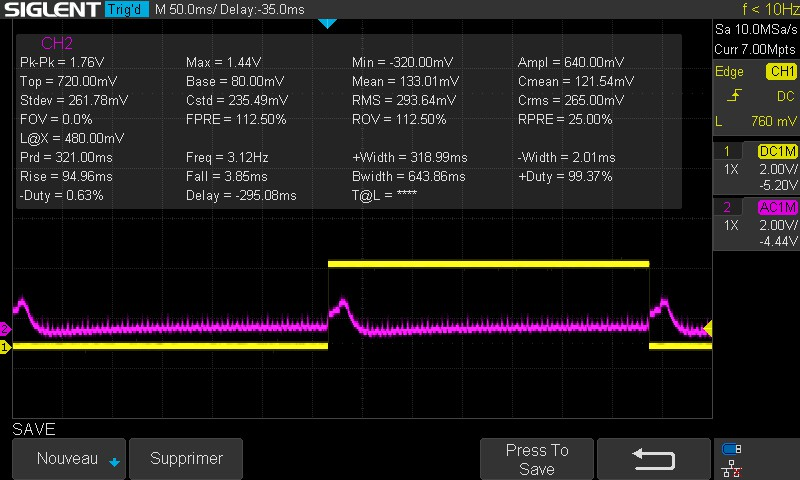
\includegraphics[width=\textwidth]{esp32_signal.jpg}
    \caption{Signals coming from the system. The yellow signal is the signel generated by the ESP32 (PWM). The purple one is the signal that we capture at the output of the filter. This signal is the one that goes in the Plant.} 
    \vspace{0.1cm}
    \label{fig:esp_32_signal}
\end{figure}



% 1. Technical Performance Testing

%     Accuracy of Plant Signal Capture: Measure how effectively the electronic filter captures changes in the plant's impedance, capacitance, and inductance when touched. This can be done by comparing sensor output data with known interactions to determine precision.
%     System Responsiveness: Test the responsiveness of the ESP32 microcontroller to human interaction with the plant. Evaluate the delay (latency) between the interaction and the corresponding sensor reading.
%     Signal Integrity: Assess the quality of the signals captured, ensuring that they are free from noise and distortion. Testing under varying environmental conditions (e.g., humidity, temperature) could be useful to ensure robustness.

% 2. User Study (Usability Testing)

%     Human Interaction Evaluation: Conduct controlled experiments to observe how users interact with different plant species, as detailed in the thesis. Participants can be asked to engage with the plants intuitively, and the interactions can be categorized as in the existing user study (e.g., pinch, grasp, slide). This helps evaluate the naturalness and intuitiveness of the plant as an interface.
%     User Satisfaction: Gather qualitative feedback from users on their experience interacting with the plants and the system's ability to translate their touch into meaningful sound. Surveys or interviews can help measure how engaging and satisfying the interaction feels.
%     Cross-species Comparison: Extend the existing user study to a wider variety of plants to ensure the system's adaptability across different plant types.

% 3. Sonification Quality

%     Audio Feedback Appropriateness: Evaluate the correlation between plant interaction and sound output. Test whether users perceive the generated sound as natural and whether different interactions (e.g., light touch vs. strong grasp) produce distinguishable auditory outputs. This could be assessed with a mixed-methods approach (e.g., user ratings and auditory analysis).
%     Sound Quality: Measure the quality of the sound generated by the embedded DAC and amplifier in terms of clarity, volume, and distortion.

% 4. System Stability and Scalability

%     Stress Testing: Test how the system behaves under continuous use and under varying loads (e.g., multiple touches in rapid succession). This will assess the system’s durability and resistance to breakdowns.
%     Scalability: Investigate whether the system can handle an increased number of sensor connections (additional plants) without performance degradation. This can be done by adding more plants and monitoring the system's response.

\subsection{Discussion}

The final product is an embedded device that include signal filtering, wireless communication and embedded sonification.


% To improve the device, the PCB could be reduced in size using a surface mounted device (SMD) ESP32 instead of a DevKit.
% I already started to work on a new version of the device. This version is only designed on Kicad and not prototyped.
% The rest of circuit is similar. 

%TODO: Add a schematic of the new PCB


A better audio amplifier could be explored in order to reduce the distortion of the sound.
Adding an external digital to analog converter is also a possibility in order to upgrade the output. However,
this possibility adds new components that will increase the size. Exploring the I2S protocol opens better output.
The I2S protocol is a protocol  %TODO: Talk quickly about I2S protocol


\subsection{Conclusion}

In conclusion, the standalone electronic system demonstrates significant potential in transforming natural plants into interactive bio-sensors, using the capabilities of a powerful microcontroller like the ESP32. The system's ability to capture plant responses to human touch and translate them into digital data is made possible by its efficient electronic interface. This architecture enables real-time interaction and offers new approach to human-plant interaction. This is also driving research into the use of plants' natural capacities as sensors. However, despite the microcontroller's strengths, the system still has notable limitations.

One major challenge lies in the sonification process, where the system struggles with producing high-quality, nuanced sound outputs due to the basic 8-bit DAC and limited audio amplification. Additionally, the data processing capabilities of the standalone device are limited, restricting the complexity of interactions it can detect and interpret. The sensor accuracy also has room for improvement, particularly in capturing fine-grained variations in plant interaction, which could taint the overall user experience and reduce the immersion.

To overcome these standalone limitations, a more sophisticated architecture is required. By connecting multiple devices in a distributed system, the Internet of Plants approach can enhance the processing power, improve sonification through external software, and allow for more complex data analysis. It could unlock the  full potential of plant-based sensors. The next section will explore how this expanded network can significantly enhance both the system's capabilities and user experience.